\subsection{Vorlesungskalendar mit Google Calendar}\label{ch:GC}
Entsprechend der Anforderungen A2 und A3 aus der Tabelle \vref{anf:GC} muss der Google Calendar vollständig in die Software integriert werden, um die Vorlesungen für die Kurse organisieren zu können. 
Damit die Ereignisse der jeweiligen Google Calendar angezeigt werden können, muss ein Kalendar in React implementiert werden. 

\subsubsection{Einbindung des DevExtreme React Scheduler}
Der \textit{DevExtreme React Scheduler}\footnote{\url{https://devexpress.github.io/devextreme-reactive/react/scheduler/}} ist ein Komponente für Material-UI, die einen Kalendar für React bereitstellt. 
Das Erscheinungsbild des React Schedulers ist von dem Google Calendar inspiriert und ist benutzerfreundlich gestaltet.\autocite[Vgl.][]{ReactScheduler} 
Neben Funktionalitäten wie beispielsweise Drag-und-Drop-Operationen sowie unterschiedliche Anzeigeoptionen, ist insbesondere die Anbindung und Integration eines Google Calendars über geeignete Schnittstellen ausschlaggebend für die Entscheidung zur Verwendung der Komponente. 

In Abbildung \vref{fig:ReactScheduler} ist eine Übersicht mit erklärenden Ergänzungen über den implementierten und konfigurierten React Scheduler dargestellt. 
Zur Verwendung des React Schedulers wird ein Package und entsprechende Abhängigkeiten von NPM eingebunden.\footnote{\url{https://www.npmjs.com/package/@devexpress/dx-react-scheduler}}
Weitere Informationen zur Einbindung sowie Konfiguration des Kalendars sind in der Dokumentation von DevExtreme gegeben.\footnote{\url{https://devexpress.github.io/devextreme-reactive/react/scheduler/docs/guides/getting-started/}}
\begin{figure}[H]
	\centering 
	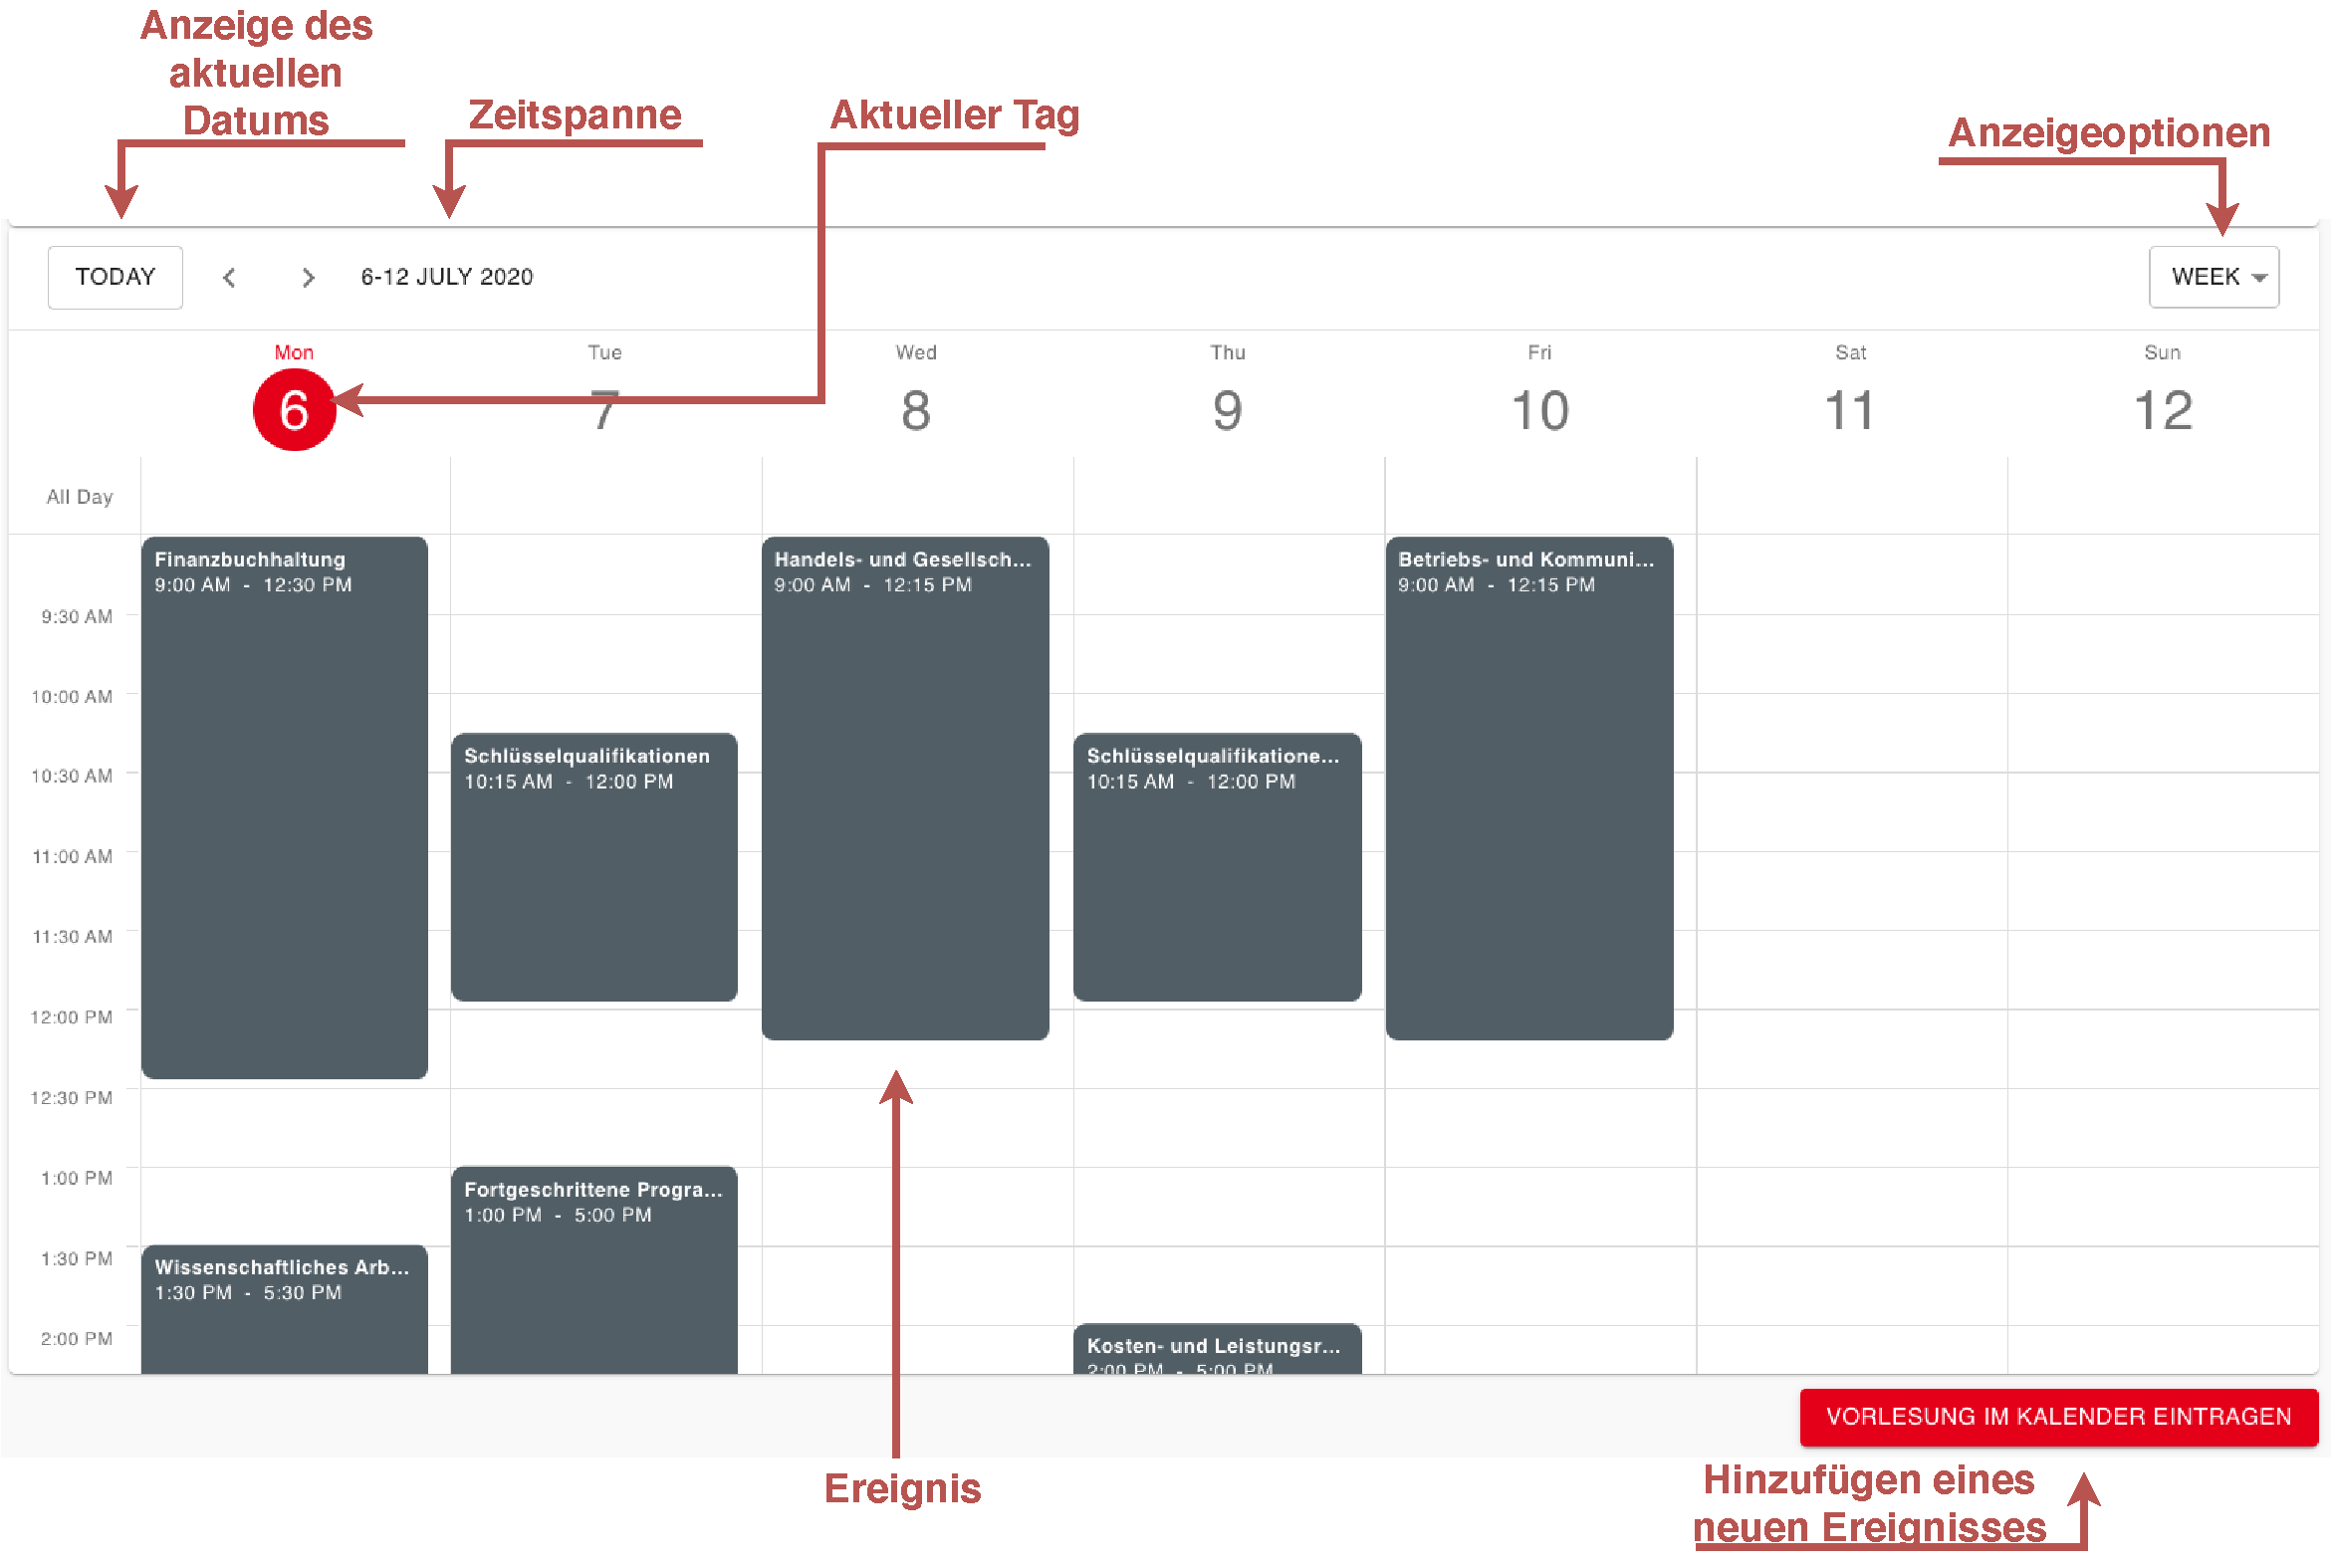
\includegraphics[width=\textwidth]{img/FrontEnd/ReactCalendar.pdf}
	\caption[Übersicht des React Schedulers]{\label{fig:ReactScheduler}Übersicht des React Schedulers\footnotemark}
\end{figure}
\footnotetext{Eigene Bildschirmaufnahme mit erklärenden Ergänzungen.}

\subsubsection{Initialisierung und Verbindung des Google Calendars}
Der Google Calendar ermöglicht eine Anbindung an das System über eine \ac{API}.
Damit die Inhalte eines Google Calendars über die Google Calendar \ac{API}-Schnittstelle\footnote{\url{https://developers.google.com/calendar/v3/reference}} angefragt und in dem React Scheduler angezeigt werden können, müssen die Anfragen über einen Token authentifiziert werden. 
Hierfür wird OAuth 2.0 verwendet, um die Authentifizierung durchzuführen.\autocite[Vgl.][]{GCApi} 

In einer eigenen JavaScript-Datei \texttt{apiHandlerGoogleCalendar.js} wird der Token bei den Anfragen, die in dem Unterkapitel \vref{ch:InteraktionGC} näher erläutert werden, mitgegeben. Dieser Token wird nach einem einmaligen Bestätigen des Zugriffs auf den Google Calendar erstellt und hinterlegt. 
Mit einem validen Token werden die Anfragen an die Google Calendar-\ac{API} genehmigt und die Inhalte des jeweiligen Kalendars an die Anwendung übertragen. Die erhaltenen Inhalte werden umformatiert und in dem React Scheduler angezeigt.


\subsubsection{Interaktion mit dem Kalendar}\label{ch:InteraktionGC}
Zur Funktionalität des Kalenders werden drei unterschiedliche Interaktionen mit dem Google Calendar benötigt: das Hinzufügen, das Ändern sowie das Löschen von Ereignissen. Im Folgenden werden die Anfragen an die REST-\ac{API} an die Google Calendar-\ac{API} näher beschrieben.

\textbf{Hinzufügen von Ereignissen}\newline
In dem React Scheduler können neue Ereignisse in dem Kalender hinzugefügt werden.
In Abbildung \vref{fig:AddReactScheduler} ist das Dialog-Fenster, welchen nach dem Drücken des Hinzufügebuttons erscheint, abgebildet.
\begin{figure}[H]
	\centering 
	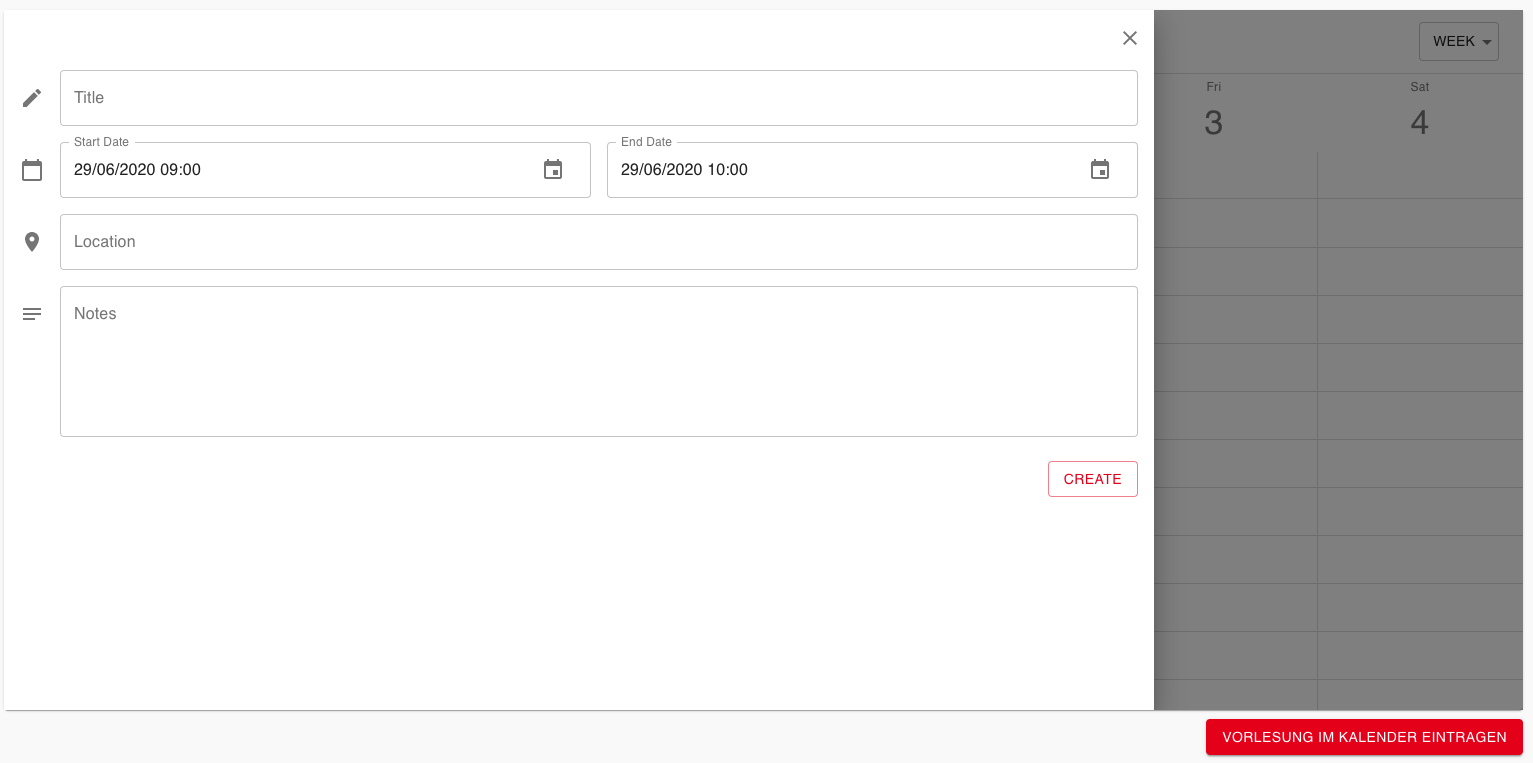
\includegraphics[width=10cm]{img/FrontEnd/GCAdd.png}
	\caption[Erstellen eines Ereignisses im React Scheduler]{\label{fig:AddReactScheduler}Erstellen eines Ereignisses im React Scheduler\footnotemark}
\end{figure}
\footnotetext{Eigene Bildschirmaufnahme.}

Zusätzlich zu den abgebildeten Inhalten werden die Kalendar-ID und der Token bei der PUSH-Anfrage übermittelt. Hierbei wird die Bibliothek \textit{GAPI} von Google verwendet, die eine einfache Verbindung mit der \ac{API} über browserseitiges JavaScript ermöglicht. 
%In dem Code-Auszug in \vref{lst:insertEvent} ist die Anfrage zum Hinzufügen eines Ereignisses abgebildet und die Übermittlung der entsprechenden Daten ersichtlich.
Eine detaillierte Dokumentation dieser Anfrage ist in der Schnittstellenbeschreibung der Google Calendar \ac{API} gegeben.\footnote{\url{https://developers.google.com/calendar/v3/reference/events/insert}}

%TODO Formatting and Coloring JavaScript-Code
%\lstset{language=JavaScript}
%\begin{lstlisting}[caption={Anfrage zum Hinzufügen eines Ereignisses}, label={lst:insertEvent}]
%function handleAppointmentInsert(insertAppointmentData, gapi) {
%  let event = {
%    'summary': insertAppointmentData.title,
%    'location': insertAppointmentData.location,
%    'description': insertAppointmentData.notes,
%    'start': {
%      'dateTime': new Date(insertAppointmentData.startDate),
%      'timeZone': Intl.DateTimeFormat().resolvedOptions().timeZone
%    },
%    'end': {
%      'dateTime': new Date(insertAppointmentData.endDate),
%      'timeZone': Intl.DateTimeFormat().resolvedOptions().timeZone
%    },
%  }
%
%  var request = gapi.client.calendar.events.insert({
%    'calendarId': creds.calenderID,
%    'resource': event
%  });
%
%  request.execute(function (response) {
%    if (response.error || response == false) {
%      alert('Error');
%    } else {
%      alert('Success');
%    }
%  });
%}
%\end{lstlisting}

\textbf{Ändern von Ereignisssen}\newline
Vorhandene Ereignisse können ebenfalls bearbeitet werden, indem die entsprechende Veranstaltung ausgewält und der Bearbeiten-Button auf dem erscheinenden Popup, welches in Abbildung \vref{fig:GCPopup} dargestellt ist, geklickt wird. 
\begin{figure}[H]
	\centering 
	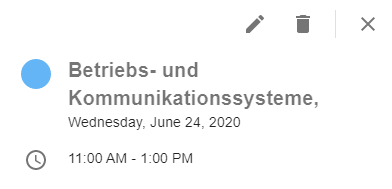
\includegraphics[width=6cm]{img/FrontEnd/GCPopup.png}
	\caption[Popup eines Ereignisses im React Scheduler]{\label{fig:GCPopup}Popup eines Ereignisses im React Scheduler\footnotemark}
\end{figure}
\footnotetext{Eigene Bildschirmaufnahme.}

Zur Änderung der Daten wird eine \ac{API}-Anfrage mit der Methode \textit{update} verwendet.\footnote{\url{https://developers.google.com/calendar/v3/reference/events/update}} 
Diese ist vom Aufbau ähnlich zu der zuvor vorgestellten \textit{insert}-Methode.

\textbf{Löschen von Ereignissen}\newline
Zusätzlich können Ereignisse in dem Google Calendar gelöscht werden, indem die Funktionalität, ebenfalls in Abbildung \vref{fig:GCPopup} abgebildet, genutzt wird. 
Zur Durchführung dieser Operation wird das Event \textit{delete} verwendet, wobei lediglich die Calendar-ID sowie die Event-ID übermittelt wird.\footnote{\url{https://developers.google.com/calendar/v3/reference/events/delete}}   
In dem Code-Ausschnitt \vref{lst:deleteEvent} ist die Erstellung der Delete-Anfrage abgebildet.

%TODO Formatting and Coloring JavaScript-Code
\lstset{language=JavaScript}
\begin{lstlisting}[caption={Anfrage zum Löschen eines Ereignisses}, label={lst:deleteEvent}]
function handleAppointmentDelete(deleteAppointmentId, gapi) {
  var request = gapi.client.calendar.events.delete({
    'calendarId': creds.calenderID,
    'eventId': deleteAppointmentId
  });

  request.execute(function (response) {
    if (response.error || response == false) {
      alert('Error');
    } else {
      alert('Success');
    }
  });
}
\end{lstlisting}

%\subsubsection{Ausblick}
%Mit dieser Integration der Inhalte des Google Calendars, können die Inhalte dargestellt und verändert werden. 
%Durch die Schnittstellen-Kommuniktaion ist jedoch ein paralleles Bearbeiten des Google Calendars, in der vorliegenden Anwendung sowie in dem Google Calendar direkt, möglich. 
%Dieses Szenario ist jedoch als sehr selten

%\begin{itemize}
%	\item Google Calendar \ac{API} 
%		\subitem \url{https://developers.google.com/calendar}
%	\item Verwendung: DevExtreme React Scheduler 	
%		\subitem \url{https://www.npmjs.com/package/@devexpress/dx-react-scheduler} 
%		\subitem \url{https://devexpress.github.io/devextreme-reactive/react/scheduler/}
%	\item Anzeigen
%	\item Termine verändern
%	\item Termine erstellen
%\end{itemize}
